\chapter{Diseño Hardware}
\label{diseño_hardware}

\paragraph{} El diseño hardware ha sido comprometido por el reducido tiempo de trescientas (300) horas dedicadas a este trabajo de fin de grado.

\section{Pantalla}
\paragraph{} La idea era desarrollar sobre una plataforma lo mas barata posible siendo la pantalla el componente más caro del mismo, y el que se pretendía minimizar al máximo con el uso de la pantalla de tinta electrónica \textit{ED060XD4} (figura \ref{fig:tfg:03:kindle}) la cual se puede obtener por quince (15) euros.

\paragraph{} Este precio es debido a que se manufactura en masa como componente principal del famoso producto \textit{amazon kindle}. Este componente trae con el las consecuencias de que sea hecho a medida para este producto, siendo todos sus datos técnicos a falta de temperaturas de operación, totalmente privativos, dificultando el desarrollo.

\paragraph{} Es por este motivo por el que se ha seleccionado la pantalla \textit{4.2inch e-Paper Module} de \textit{Waveshare} (figura \ref{fig:tfg:03:waveshare}), siendo su integración con el producto final muchísimo más fluida debido a la aportación de drivers, pinout y una ficha técnica completa, directamente por el fabricante, a costa del precio de cuarenta (40) euros.

\paragraph{} Gracias a la elección de esta pantalla, se podrá hacer uso de dos colores a demás del fondo blanco de la pantalla, siendo negro y rojo los colores, dependiendo de la tensión aplicada a cada celda, mientras que la pantalla anteriormente descrita no ofrece esta posibilidad, esto ayudará a construir una interfaz más clara para el usuario final del dispositivo físico.

\paragraph{} Una característica que no posee la pantalla de \textit{waveshare} es la capacitiva, o táctil, la cual el display de \textit{kindle} si que posee, esto seria una característica que aportaría mucho valor al producto, pudiendo diseñar interfaces más complejas.

\begin{figure}[!htb]
    \centering
    \begin{subfigure}[b]{.475\textwidth}
        \centering
        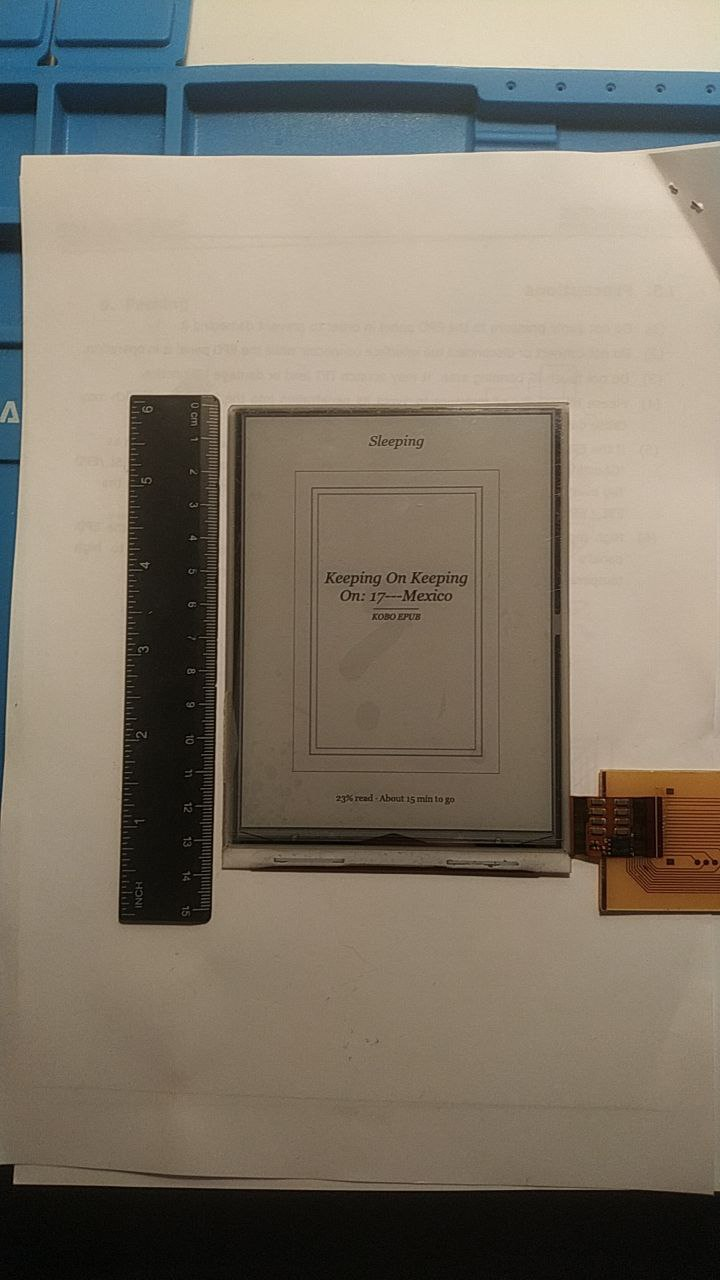
\includegraphics[width=1\textwidth, trim={0 400 0 400}, clip]{tfg/figuras/03_diseño_hardware/pantalla/kidnle.png}
        \caption{Pantalla ED060XD4 del Amazon kindle}
        \label{fig:tfg:03:kindle}
    \end{subfigure}
    \hfill
    \begin{subfigure}[b]{.475\textwidth}
        \centering
        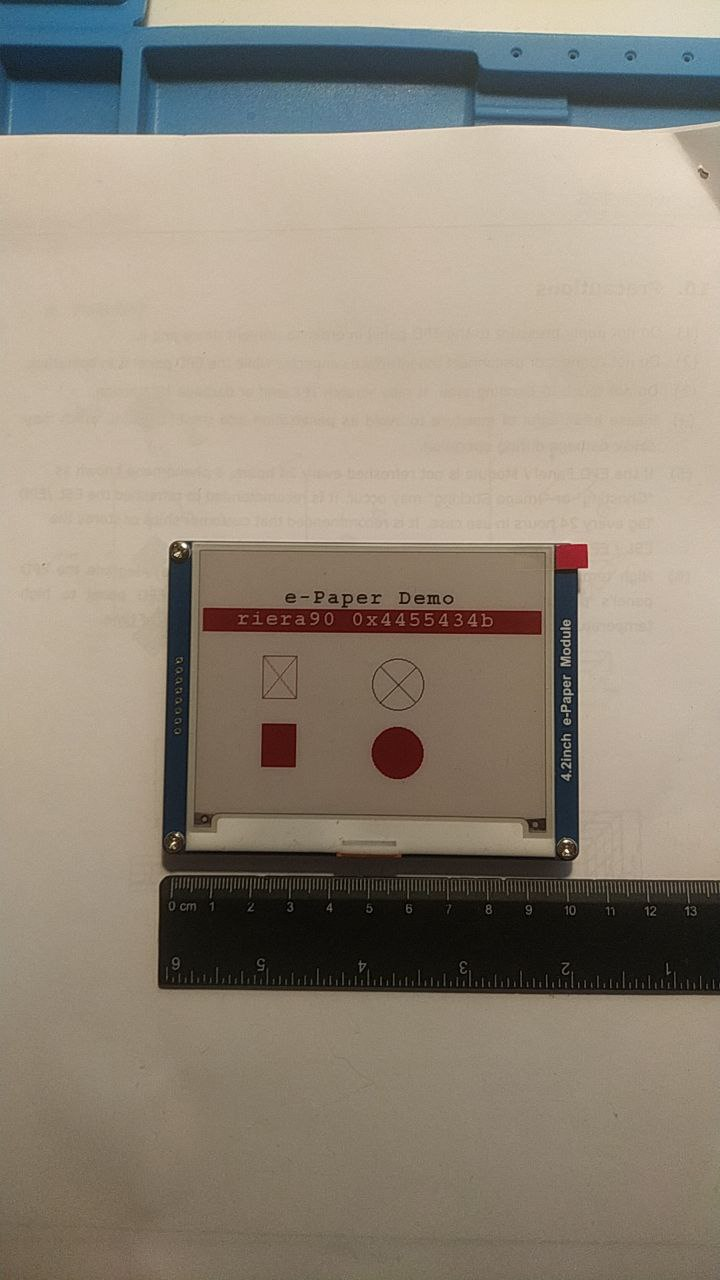
\includegraphics[width=1\textwidth, trim={0 300 0 500}, clip]{tfg/figuras/03_diseño_hardware/pantalla/waveshare.png}
        \caption{Pantalla Waveshare de 4.2 pulgadas}
        \label{fig:tfg:03:waveshare}
    \end{subfigure}
    \caption{Preselección de microcontroladores}
    \label{fig:tfg:03:pantallas}
\end{figure}


\section{Microcontrolador}

\paragraph{} Entre los microcontroladores valorados están el \textit{STM32}, el \textit{ATMega328P}, el modulo \textit{ESP8266-12F} y el propio \textit{ESP8266EX}, mostrados en la figura \ref{fig:tfg:03:microcontroladores}. Estos microcontroladores son escogidos por ser adecuados al proyecto y de tenerlos en estocaje, puesto que la crisis de integrados y los tiempos de espera para su compra podrían atentar a la realización de este proyecto.

\begin{figure}[!htb]
    \centering
    \begin{subfigure}[b]{.475\textwidth}
        \centering
        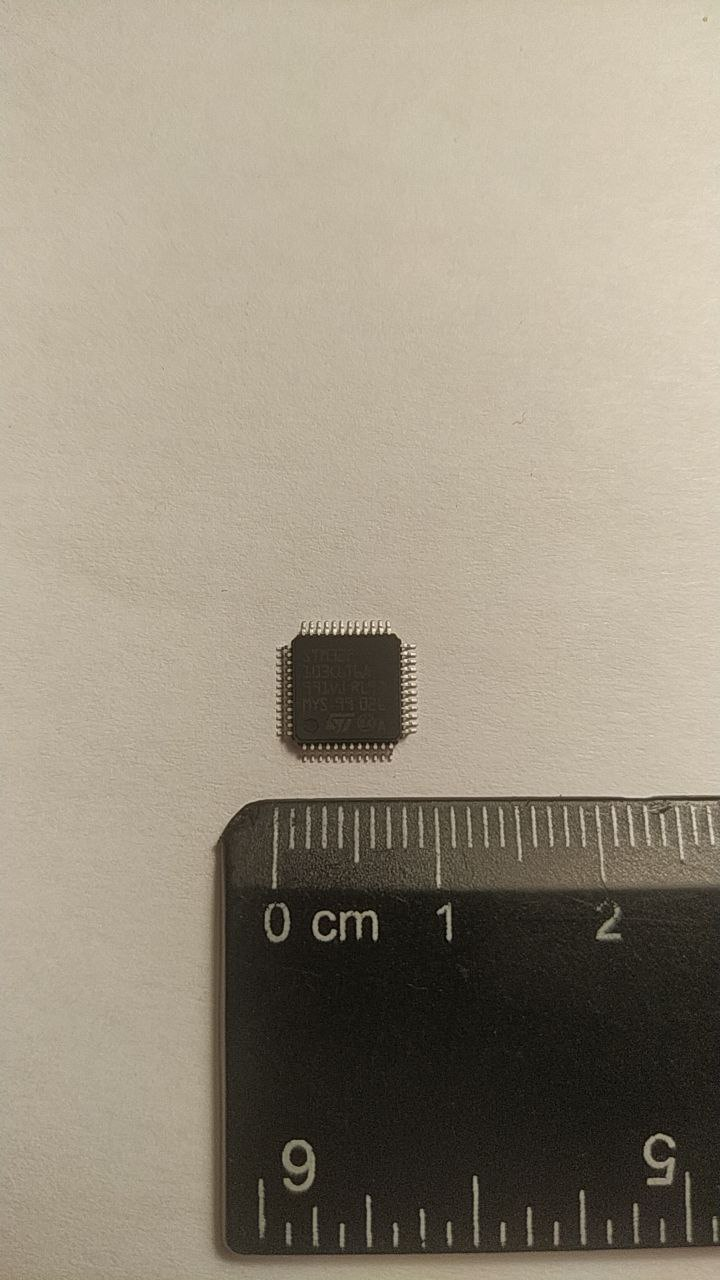
\includegraphics[width=1\textwidth, trim={0 350 0 450}, clip]{tfg/figuras/03_diseño_hardware/microcontroladores/stm32.png}
        \caption{Microcontrolador STM32}
        \label{fig:tfg:03:stm32}
    \end{subfigure}
    \hfill
    \begin{subfigure}[b]{.475\textwidth}
        \centering
        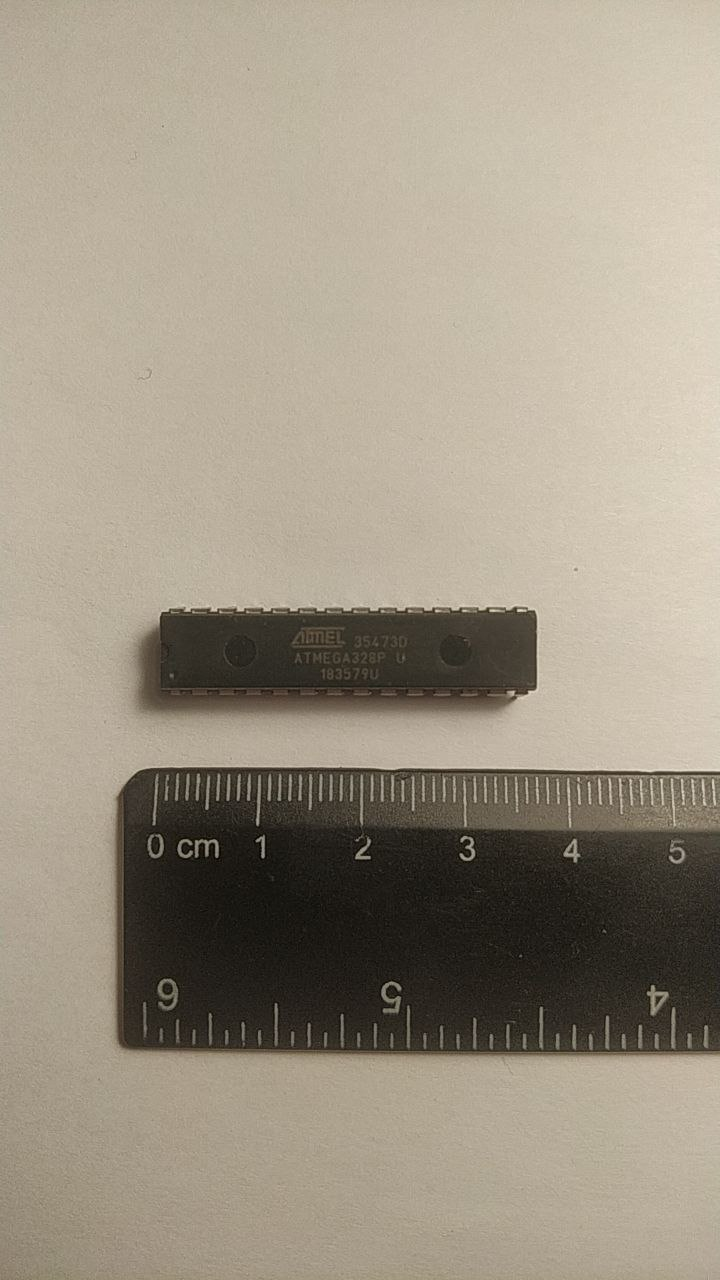
\includegraphics[width=1\textwidth, trim={0 400 0 400}, clip]{tfg/figuras/03_diseño_hardware/microcontroladores/atmega.png}
        \caption{Microcontrolador ATMega328P}
        \label{fig:tfg:03:atmega328p}
    \end{subfigure}
    \vskip\baselineskip
    \begin{subfigure}[b]{.475\textwidth}
        \centering
        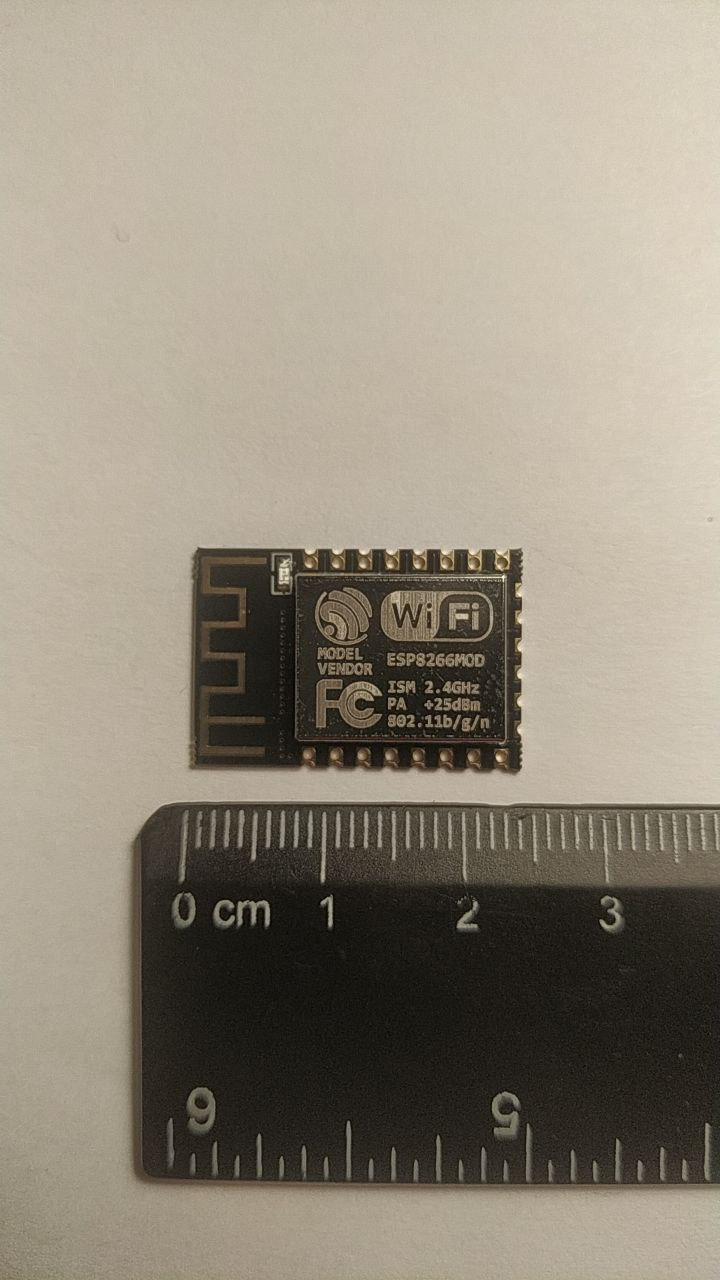
\includegraphics[width=1\textwidth, trim={0 350 0 450}, clip]{tfg/figuras/03_diseño_hardware/microcontroladores/esp8266-12f.png}
        \caption{Microcontrolador ESP8266EX en formato 12F}
        \label{fig:tfg:03::esp8266-12f}
    \end{subfigure}%
    \hfill
    \begin{subfigure}[b]{.475\textwidth}
        \centering
        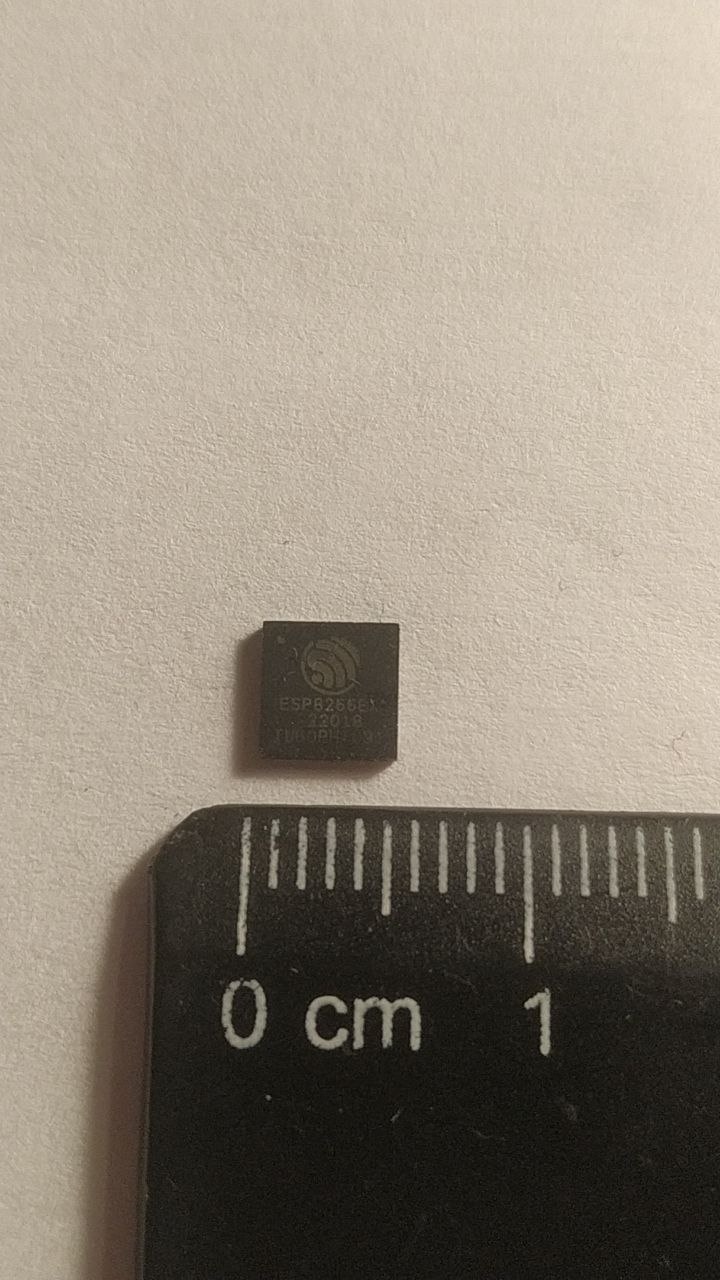
\includegraphics[width=1\textwidth, trim={0 325 0 475}, clip]{tfg/figuras/03_diseño_hardware/microcontroladores/esp8266ex.png}
        \caption{Microcontrolador ESP8266EX}
        \label{fig:tfg:03:esp8266ex}
    \end{subfigure}%
    \caption{Preselección de microcontroladores}
    \label{fig:tfg:03:microcontroladores}
\end{figure}

\paragraph{} De estos microcontroladores se requiere que se conecten a un punto de acceso wifi, como se desea simplificar al máximo el numero de componentes del circuito, reduciendo así posibles fallos y facilitando el diagnostico del sistema, se reduce la selección a los microcontroladores \textit{ESP8266-12F} y \textit{ESP8266EX}, puesto que tienen incorporada la conectividad a WiFi y la pila TCP implementado en hardware.

\paragraph{} Entre estos dos, se escoge el paquete del \textit{ESP8266-12F} por el motivo de resultar en un circuito de tamaño más reducido, esto parece contradictorio, pero si tomamos en cuenta los componentes que necesitan cada uno para su correcto funcionamiento, la huella del \textit{ESP8266EX} es mayor, puesto que el autor no posee componentes de tamaño tan reducido como los que monta el \textit{ESP8266-12F}, a demás de contar con un escudo RF para reducir interferencias.

\paragraph{} En cuestión a la programación y características eléctricas, ambos son idénticos, de tal manera que en un futuro si se desea, mediante un simple rediseño de la placa el cambio entre estos microcontroladores es posible, ya sea por miniaturización o por cuestiones económicas.

\section{Sensorica}

\paragraph{} Para poder interactuar con el usuario, los dispositivos más usados normalmente son los botones, codificadores capacitivos, potenciómetros o sensores capacitivos, a continuación se explican cada uno de ellos en detalle:

\paragraph{} Los botones pueden ser el sensor más común para interaccionar con el usuario, por su simpleza y sensación táctil son fáciles e intuitivos de usar, pero tienen un desgaste inherente a su naturaleza y requieren de reemplazo aun con su correcto uso. Para asegurarnos que dicho reemplazo suceda lo más tarde posible, siempre se puede realizar uso de un botón más robusto, pero dicha robustez requiere que el componente sea de mayor dimensión. Esto se puede observar en las figuras \ref{fig:tfg:03:boton_smd}, \ref{fig:tfg:03::boton_tht} y \ref{fig:tfg:03:boton_grande_tht}

\paragraph{} Tanto los potenciómetros como codificadores rotacionales son sensores cuya función es transmitir información dependiendo de el ángulo de giro o el numero de grados girado respectivamente, aunque interesantes, este tipo de sensores es más adecuado a una interfaz más ágil que una pantalla de tinta electrónica, donde el usuario puede realizar múltiples acciones antes de que se pueda actualizar la pantalla una única vez, por eso este sensor se desecha de la selección.


 \paragraph{} Finalmente, los sensores capacitivos como el \textit{TTP223R} (figura \ref{fig:tfg:03:ttp223r}) actúan mediante el uso de un electrodo en la placa de circuito impreso como un condensador variable con la proximidad de un dedo, activando así una señal de salida del integrado. Este tipo de sensores es inmune al desgaste mecánico, ya que no tienen ninguna pieza móvil, lo cual los hace interesante para este proyecto y motivo por el cual se seleccionan como sensor.


\begin{figure}[!htb]
    \centering
    \begin{subfigure}[b]{.475\textwidth}
        \centering
        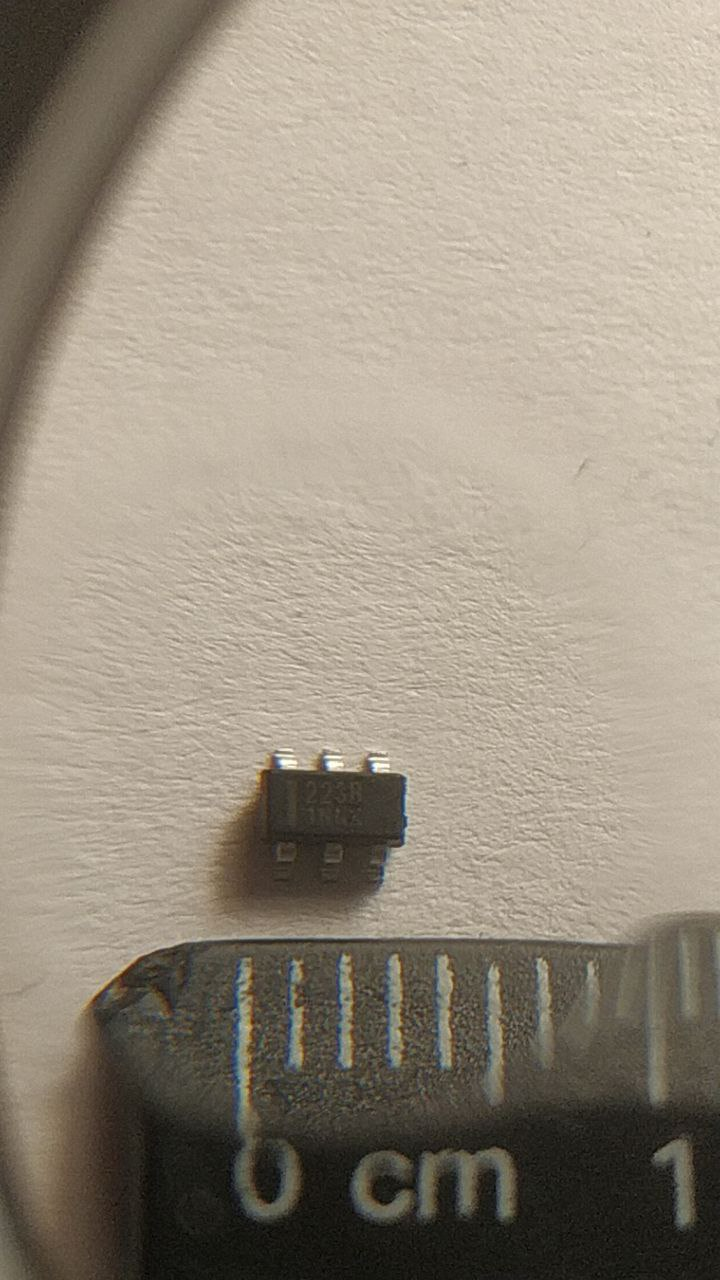
\includegraphics[width=1\textwidth, trim={0 150 0 650}, clip]{tfg/figuras/03_diseño_hardware/sensorica/ttp223r.png}
        \caption{Sensor capacitivo TTP223R}
        \label{fig:tfg:03:ttp223r}
    \end{subfigure}
    \hfill
    \begin{subfigure}[b]{.475\textwidth}
        \centering
        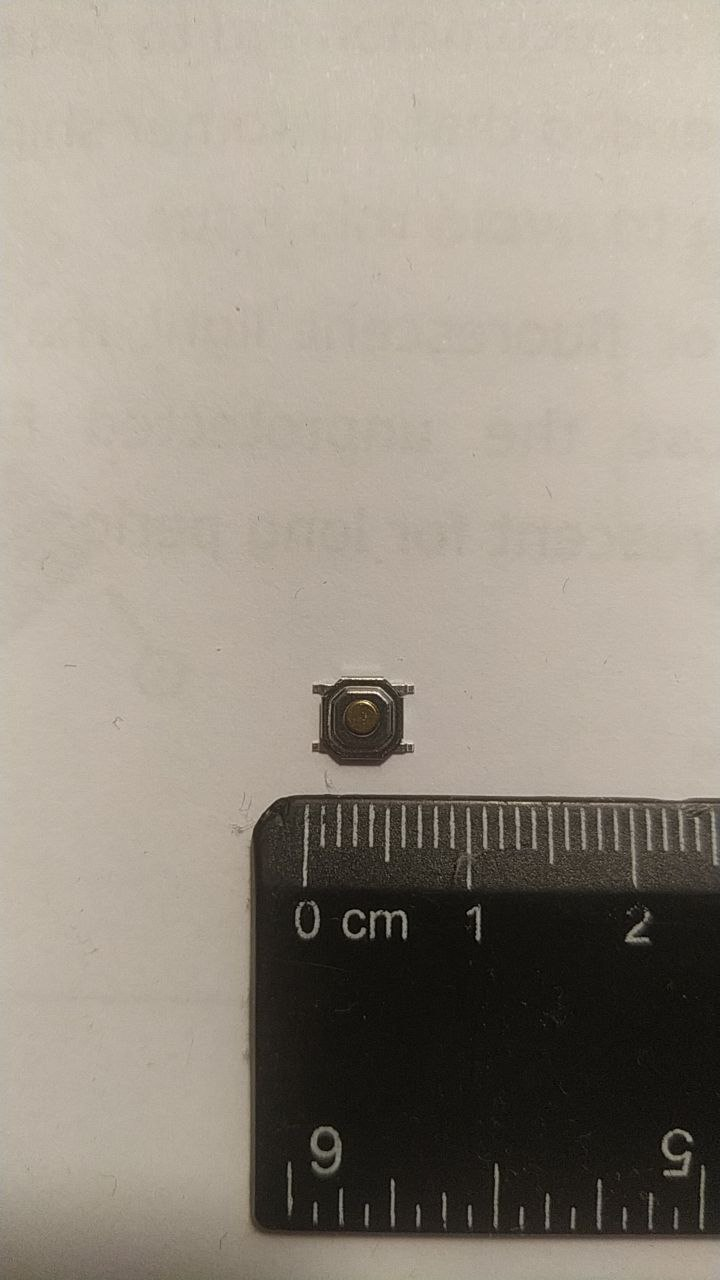
\includegraphics[width=1\textwidth, trim={0 300 0 500}, clip]{tfg/figuras/03_diseño_hardware/sensorica/boton_smd.png}
        \caption{Botón SMD}
        \label{fig:tfg:03:boton_smd}
    \end{subfigure}
    \vskip\baselineskip
    \begin{subfigure}[b]{.475\textwidth}
        \centering
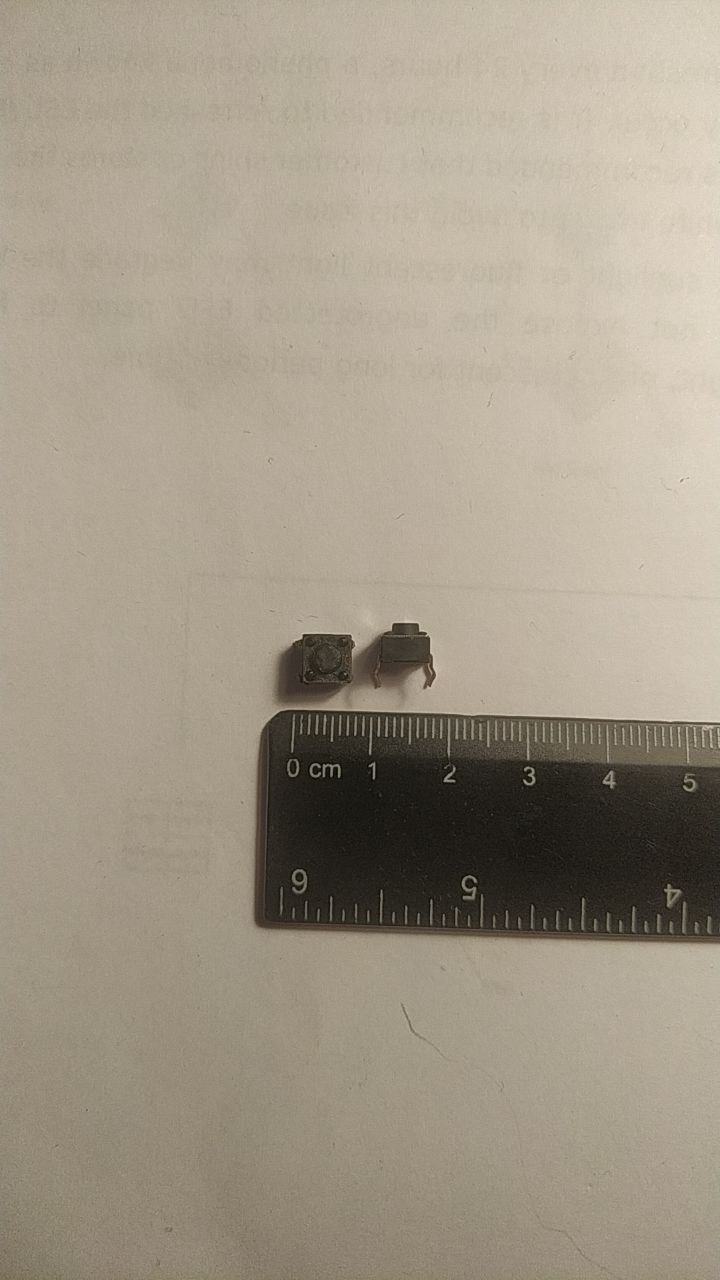
\includegraphics[width=1\textwidth, trim={0 350 0 450}, clip]{tfg/figuras/03_diseño_hardware/sensorica/boton_tht.png}
        \caption{Botón THT}
        \label{fig:tfg:03::boton_tht}
    \end{subfigure}%
    \hfill
    \begin{subfigure}[b]{.475\textwidth}
        \centering
        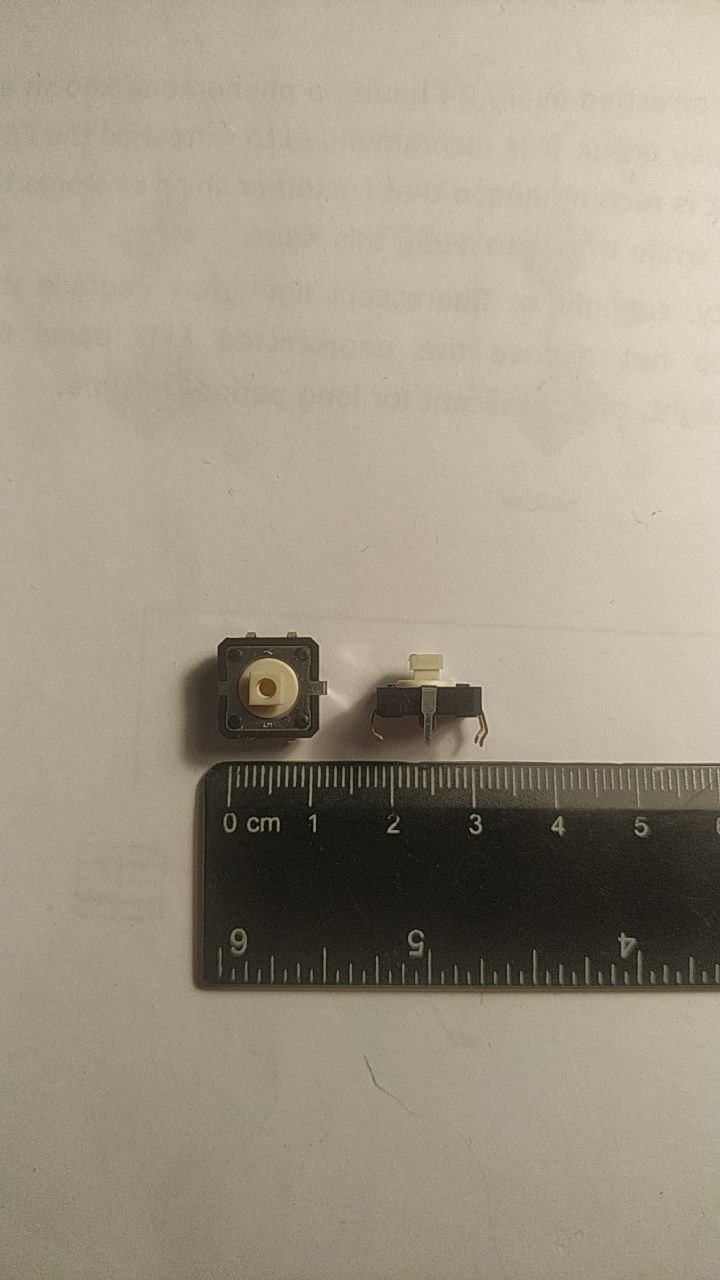
\includegraphics[width=1\textwidth, trim={0 325 0 475}, clip]{tfg/figuras/03_diseño_hardware/sensorica/boton_grande_tht.png}
        \caption{Botón THT más robusto}
        \label{fig:tfg:03:boton_grande_tht}
    \end{subfigure}%
    \vskip\baselineskip
    \begin{subfigure}[b]{.475\textwidth}
        \centering
        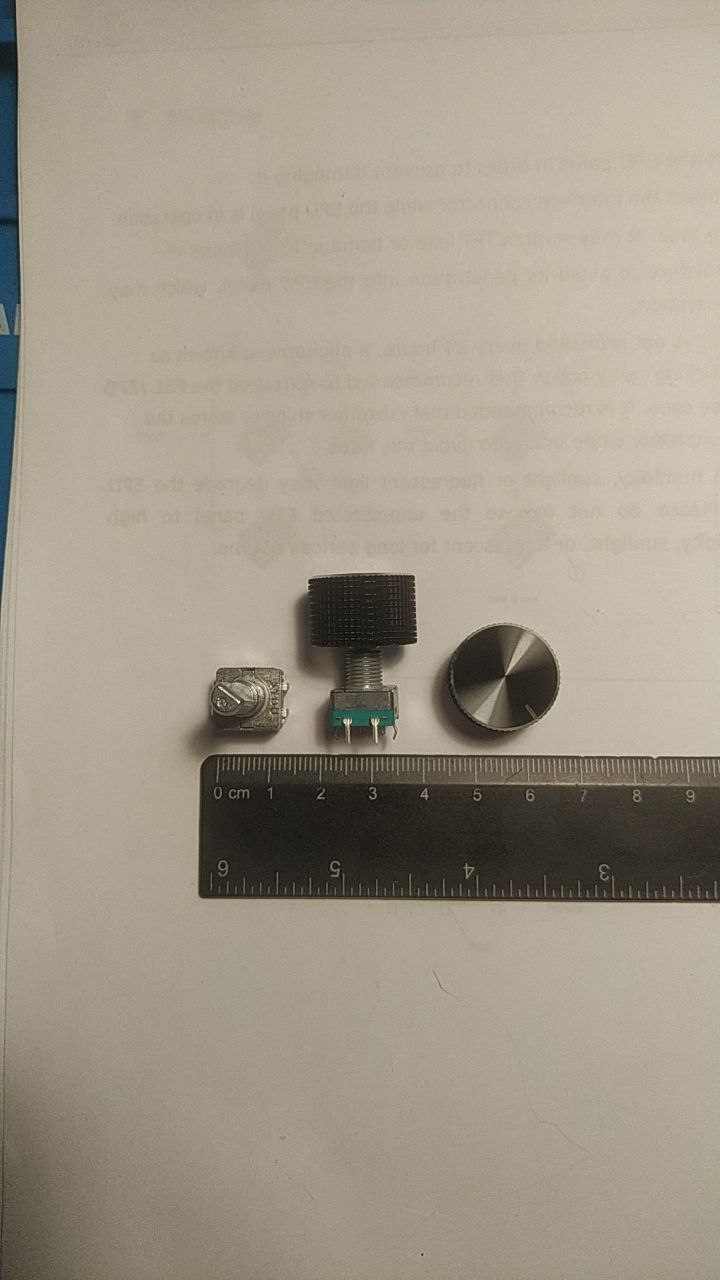
\includegraphics[width=1\textwidth, trim={0 350 0 450}, clip]{tfg/figuras/03_diseño_hardware/sensorica/encoder.png}
        \caption{Codificador rotacional}
        \label{fig:tfg:03::encoder}
    \end{subfigure}%
    \caption{Preselección de sensores}
    \label{fig:tfg:03:sensorica}
\end{figure}

\section{Regulación de voltaje}

\paragraph{} El circuito necesitará de regulación de voltaje para la alimentación tanto de la pantalla, la cual funciona a 5 voltios y para el microcontrolador \textit{ESP}, alimentado a 3.3 voltios.

\begin{figure}[!htb]
    \centering
    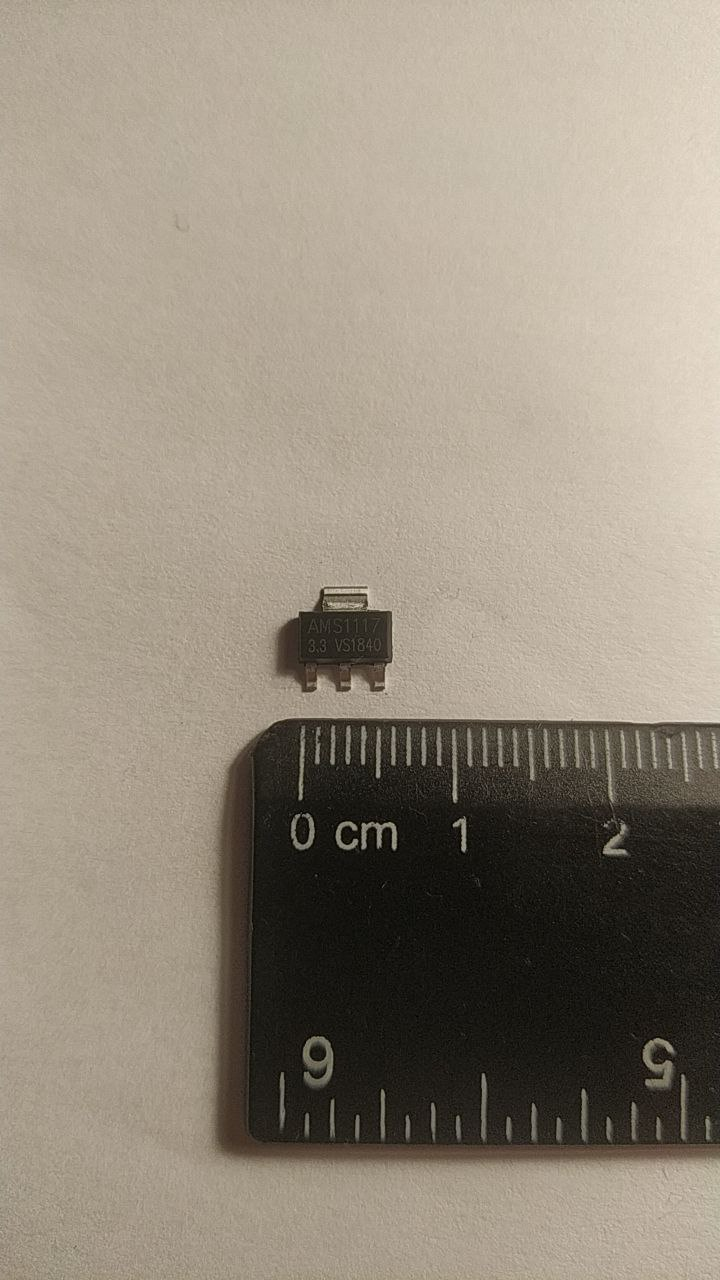
\includegraphics[width=.475\textwidth, trim={0 350 0 450}, clip]{tfg/figuras/03_diseño_hardware/reguladores/asm1117-3v3.png}
    \caption{Regulador de voltaje ASM1117 3v3}
    \label{fig:tfg:03:asm1117-3v3}
\end{figure}

\paragraph{} Para alimentar el \textit{ESP}, cuyo consumo medio rondará los microamperios, con mínimos de quinientos (500) nanoamperios y con picos de ciento setenta (170) miliamperios en su máximo consumo, se escoge el \textit{ASM1117} de 3.3 voltios (figura \ref{fig:tfg:03:asm1117-3v3}) debido a su reducida huella.

\paragraph{} Este regulador también se usará para alimentar la pantalla, modificando el voltaje de referencia a 1.7 voltios, para regular su salida a 5 voltios, los motivos son idénticos que para alimentar el \textit{ESP}, puesto que la pantalla consume extremadamente poco de media, 170 nanoamperios amperios si está en reposo, 7.2 miliamperios mientras se está actualizando.

\section{Conexionado}

\paragraph{} El conexionado de los componentes se realizará mediante un circuito impreso de dos caras, el cual se realizará a medida